\chapter{Using structured data to evaluate methods of reference-free variant calling}
\label{ch:structured}

Genotyping a sample given a set of next generation sequencing reads is a common task in biology. However, genotyping accurately and sensitively is difficult due to errors in sequencing reads. This problem is exacerbated when genotyping non-model organisms because they may lack a polished annotated genome and other prior information that is sometimes used in genotyping pipelines. Once obtained, these genotypes can be used for many things; detecting selection in a population, discovering genes and alleles that affect a particular phenotype, or comparing them to another population to attempt to understand their evolutionary history.

While accurate genotype calls are important for all these uses, accurate detection of variation is difficult even with plenty of time, money, and other auxilliary resources available. Without a high-quality genome and a large number of reads, the task becomes much harder. However, several methods have been developed to call variants directly from sequencing reads, with no additional information necessary. These methods use de bruijn graphs or similar structures to create contiguous sequences representing the genome, much like assembly. They also keep track of which samples the sequences in the graph came from. Once the graph is completed, it can be traversed to find bubble-like structures in the graph. These are locations where the sequences specific to different samples diverge briefly, then come back together. This indicates the presence of a single nucleotide polymorphism (SNP) or short insertion-deletion in one of the samples. Then, the sequences that differ can be extracted from the graph and aligned to a reference, if one exists.

There are a variety of software packages that implement reference-free variant calling in this manner. One of the first developed is an extension of the Cortex assembler and is called cortex\_var. A more recent method called DiscoSNP++ was developed which doesn't require as much RAM or CPU and allows direct VCF output after mapping the predicted variants to a genome. DiscoSNP++ has recently been updated to include a tool specifically for use with RAD-seq data. Reference-free methods do not necessarily need to use de-bruijn graphs, however. The recently developed method, Kestrel, attempts to find variants without a graph and solely considers k-mer counts. %EBWT??

I previously called genotypes in the non-model organism \textit{Eucalyptus melliodora} using both out-of-the-box and custom methods to genotype leaves sampled across the tree \parencite{orr_phylogenomic_2020}. I leveraged the sample structure to estimate false positive rates for each step in the pipeline I used. When I began that work, the available reference-free methods were not sufficiently developed to call variants with the necessary accuracy I wanted to be confident in the results. Since then, the methods have undergone more development, so I was interested in whether they would work for the same data. In this chapter, I use the reference-free variant caller DiscoSNP++ and, as before, use the structure of the data to estimate the false positive rate. I also compare the output of the caller with the set of confident variants detected using the maximum likelihood approach described in \parencite{orr_phylogenomic_2020} and implemented with DeNovoGear. %todo: cite

\section{Methods}

%adapted from /storage/2017-03-15-eucalyptus/2019-12-16-supplement/filter_steps/false-positive-rate
%scripts are in /storage/2017-03-15-eucalyptus/2020-10-05-disco
To obtain variants to compare to the variant set obtained in \cite{orr_phylogenomic_2020}, I ran the DiscoSNP++ program on the raw sequencing reads. DiscoSNP++ was run with the included run\_discoSnp++.sh shell script with the -G, -T, and -R flags set along with the pseudo-reference genome from \cite{orr_phylogenomic_2020}. This enables alignment of the detected variants to the reference and creation of a VCF from the aligned haplotypes.

DiscoSNP++ was chosen as the reference-free caller to use because it was the only one that was able to be successfully installed and run on the system I used to analyze the data. Cortex uses a custom installation script that failed to properly compile the program; it could not properly link the submodules Cortex uses. Installation of Kestrel was standardized and simple, but required too much memory for this dataset. It was run with the default 4G of memory, 8G, 64G, and 256G, but crashed each time, complaining of insufficient memory. The manual gives no advice for setting this parameter.

To understand how each filtering step previously applied to this data affected the number of variants in this set, I applied 7 of 8 of these filters to the set of variants. Prior to these filters, however, I used BCFTools to remove any site which included a "." genotype, since every sample is diploid; "./." genotypes were permitted until the second to last step. The first filter only permits variants that appear on the first 11 scaffolds of the genome; these represent the chromosomes of \textit{E. melliodora}. Variants with depth > 500 were then excluded, as higher than expected depth is a signal of alignment problems. The ExcessHet annotation could not be used for filtering, as this filter is specific to GATK. I then filtered out variants within 50bp of an indel, another indicator of alignment issues. I then removed any variant that was not a biallelic SNP, as these are more likely to be errors than true mutations. Note that this makes it impossible for this pipeline to detect heterozygous to heterozygous mutations. I then removed variants that were in repetitive regions determined by a liftover of the \textit{E. grandis} RepeatMasker annotation to the pseudo-reference. Finally, I removed all sites where any set of three replicates did not have the same genotype. I then included only sites that included a mutation (\textit{ie.} not all heterozygous) to get the final set of variants.

To visualize how each filtering step affected the overall quality of the called variants, I concatenated the variants found in each step to create a FASTA alignment of sites and used RaxML with the -f a option to search for the best-scoring maximum likelihood tree, the -m ASC\_GTRGAMMA model to use a GTR mixture model with gamma distributed rate heterogeneity and correct for ascertainment bias, and the --asc-corr lewis option to use Paul Lewis' correction for ascertainment bias. Variant concatenation is not the optimal way to infer accurate phylogenies; however, for the purposes of a visual summary of the data it is sufficient.

	% false positive and false negative calls, I estimated the number of each type of variant at each step in the filtering process and evaluated how each filter affected the resulting phylogenies constructed using the obtained set of genotypes.
To evaluate the performance of this pipeline, I estimated the number of false positives and true positives were present in the reads. Since this is an empirical dataset and the the truth is not known, I had to estimate the number of true positives and false positives. To estimate the number of false positives, I randomized 100 trees that were maximally distant from the true tree and identified the number of mutations where the variants called matched the randomized replicate structure at each filtering step. This is similar to applying the second-to-last and last set of variant filters, but using the randomized tree instead of the true tree topology. Since a real mutation should follow the true structure of the tree but are unlikely to match the structure of the randomized trees, these variants are false positives. I then assumed a similar number of false positives appear when using the true tree structure, and infer the false positive rate of the calls is equal to the false positive rate calculated using the random trees.  %Since the randomized trees are all maximally distant from the true tree, a mutation called in a randomized tree should never be present in the true tree. Assuming a true mutation is consistent with only the true tree topology, I conclude that such mutations must therefore be false positives.

True positives are difficult to estimate, and the structure of the data does little to assist in identifying true variants. I therefore use the confident set of mutation calls made in \cite{orr_phylogenomic_2020} and treat them as the set of true positives. Any calls that overlap this set are therefore classified as true positives, and the number of calls that are not present in the set are classified as false negatives. Note that, as found in \cite{orr_phylogenomic_2020}, this set has an approximate false negative rate of 30\%, so it's possible that true mutations are not classified as such under this classification scheme.


\section{Results}

DiscoSnp++ emitted a total of of 1,114,434 potential variants; however, only 951,924 of these mapped to one of the first 11 scaffolds. After applying all filters, only 4 variants were ultimately detected (see Table \ref{ev_num_variants}). Before filtering, 27 of the 90 possible confident set variants were detected; after filtering, none were. Interestingly, the estimated number of false positives are very low, with an estimated 14.55 before filtering and only 2.8 after.

\begin{table}
\begin{tabularx}{\textwidth}{>{\hsize=1.5\hsize\linewidth=\hsize}X >{\hsize=.7\hsize\linewidth=\hsize}X >{\hsize=.9\hsize\linewidth=\hsize}X >{\hsize=.9\hsize\linewidth=\hsize}X}
\toprule
\textbf{Description} & \textbf{Num} & \textbf{Estimated} & \textbf{True}\\
& \textbf{Variants} & \textbf{False Positives} & \textbf{Positives} \\
\midrule
Appears in first 11 scaffolds & 951924 & 14.55 & 27\\
Total depth <= 500 & 910361 & 5.96 & 27\\
Not within 50bp of an indel & 893535 & 5.9 & 26\\
Biallelic SNPs & 815925 & 5.68 & 26\\
Outside repeat regions & 432414 & 2.8 & 20\\
All 3 replicates match & 2150 & - & 0\\
Only variable sites & 4 & - & 0\\
\bottomrule
\end{tabularx}
\titlecaption{Number of Detected Variants After Each Filtering Step}{The number of variants detected at each filtering step. Each row introduces a new filter that applies in addition to all the filters in the above rows. A description of each filter, the number of variants remaining after the filter has been applied, the estimated number of false positives present at that point in filtering, and the number of variants that overlaps the previously estimated confident set of variants. Since the last two steps include filtering based on replicate agreement, the method for estimating the number of false positives is not applicable; in the worst case, they are identical to the number of estimated false positives in step 6. True positives were estimated using the number of variants ultimately detected in the confident set described in \cite{orr_phylogenomic_2020}, which contains 90 variants.}
\label{tbl:ev_num_variants}
\end{table}

The trees inferred from the set of variants detected at each site are shown in Figure \ref{fig:ev_filtertrees}. The second to last filtering step where variants only pass filtering if they are consistent in all three replicates and the last filtering step where variants only pass filtering if there is a mutation (\textit{ie.} not all heterozygous sites of the same genotype) both yielded the same tree, as the nonvariable sites are removed in the tree construction pipeline. Each tree structure differs significantly from the true tree, and there are few examples of all three replicates neighboring one another.

	%TODO: add RF distances from each tree to the real tree ?

\begin{figure}
\centering
\begin{tabularx}{\textwidth}{ >{\hsize=.5\hsize\linewidth=\hsize}X >{\hsize=1.5\hsize\linewidth=\hsize}X | >{\hsize=.5\hsize\linewidth=\hsize}X >{\hsize=1.5\hsize\linewidth=\hsize}X }
\toprule
Filtering Step & Tree & Filtering Step & Tree \\
\midrule
First 11 Scaffolds & 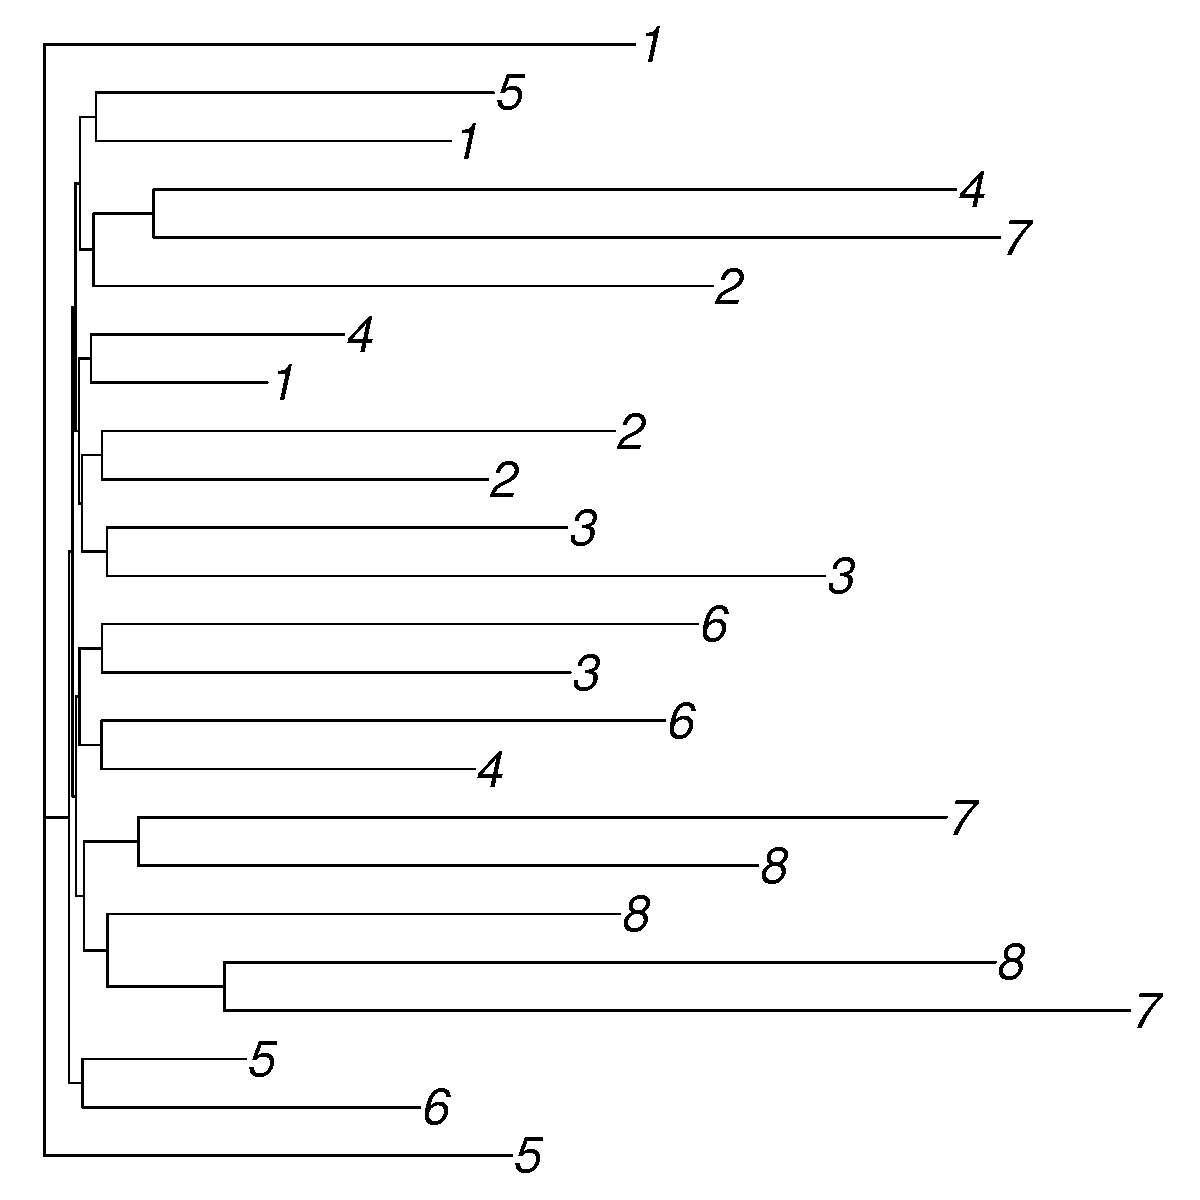
\includegraphics[width=\linewidth]{01-first-11-scaffolds.pdf} &
Depth <= 500 & 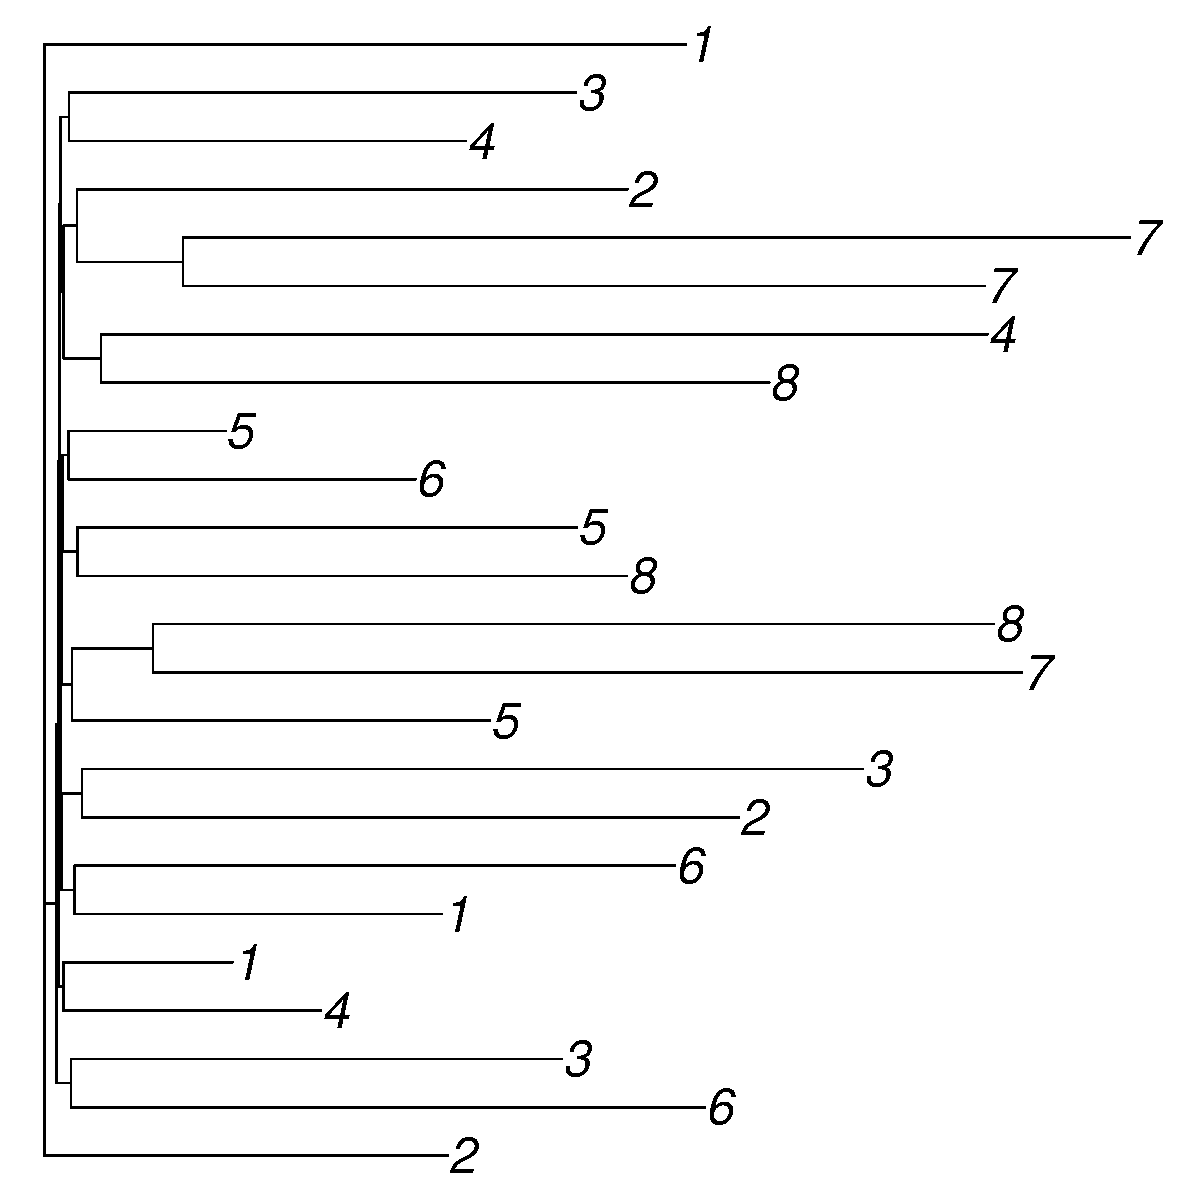
\includegraphics[width=\linewidth]{02-depth.pdf} \\
Not within 50bp of an indel & 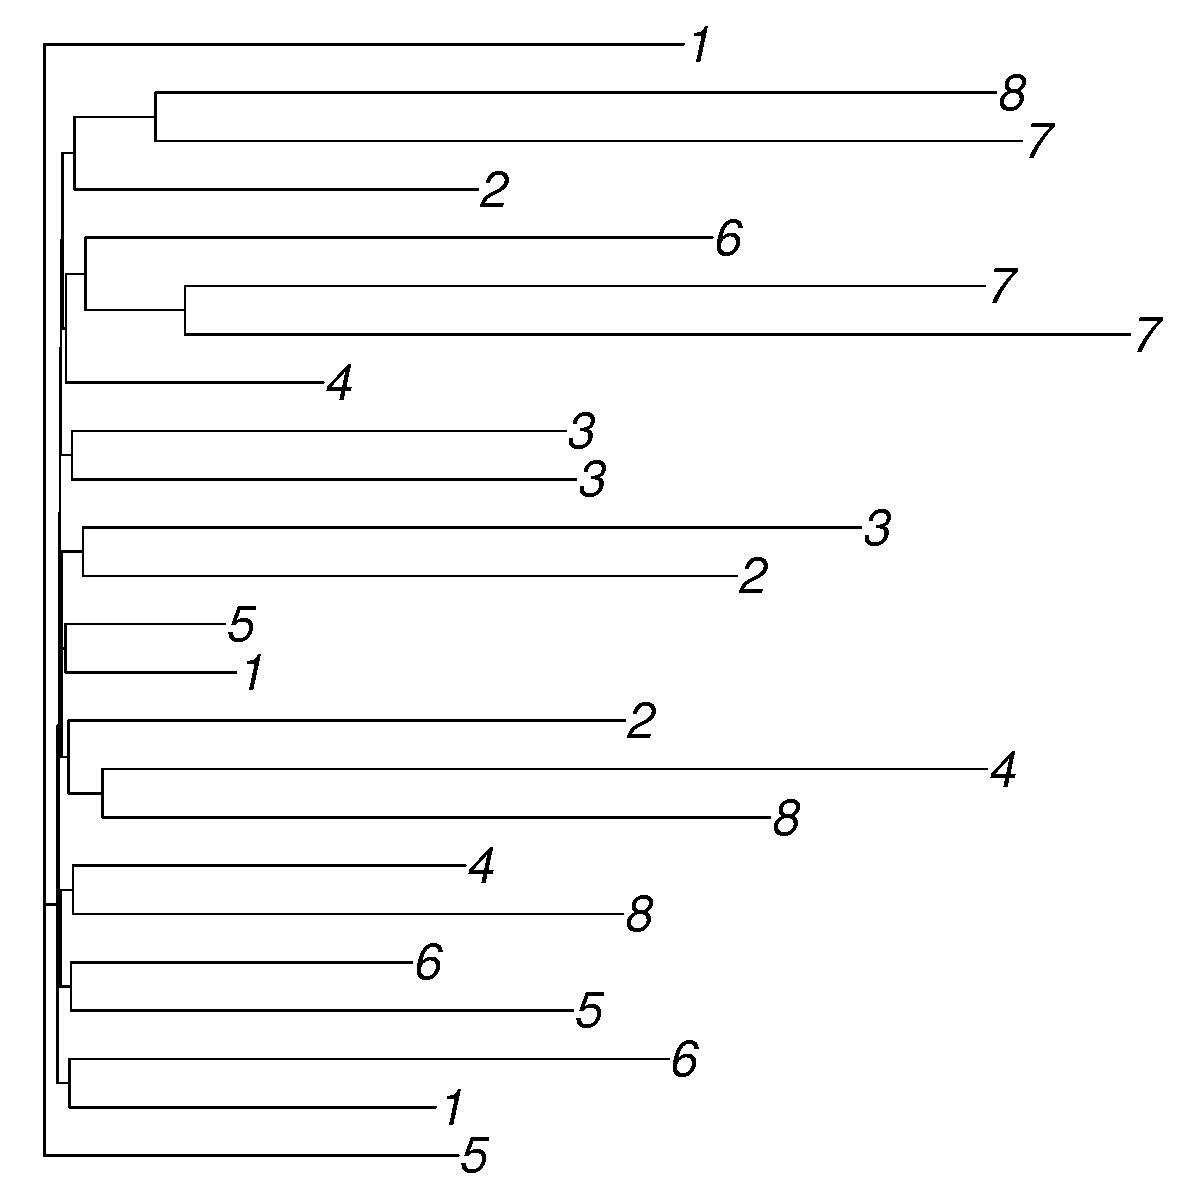
\includegraphics[width=\linewidth]{04-near-indel.pdf} &
Biallelic SNPs & 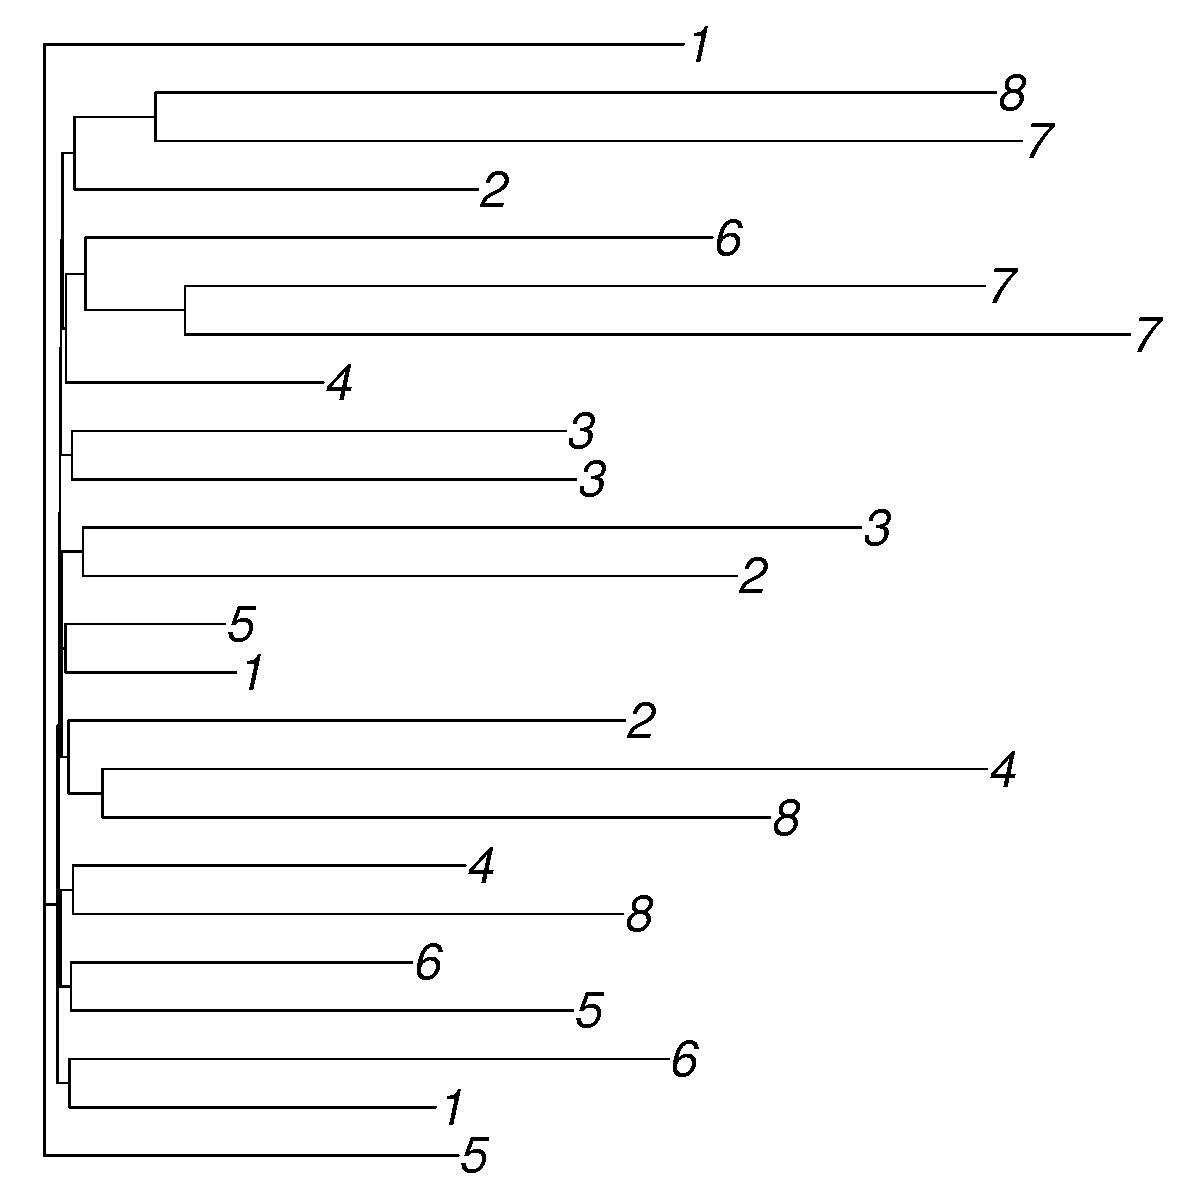
\includegraphics[width=\linewidth]{05-biallelic.pdf}\\
Outside repeat regions & 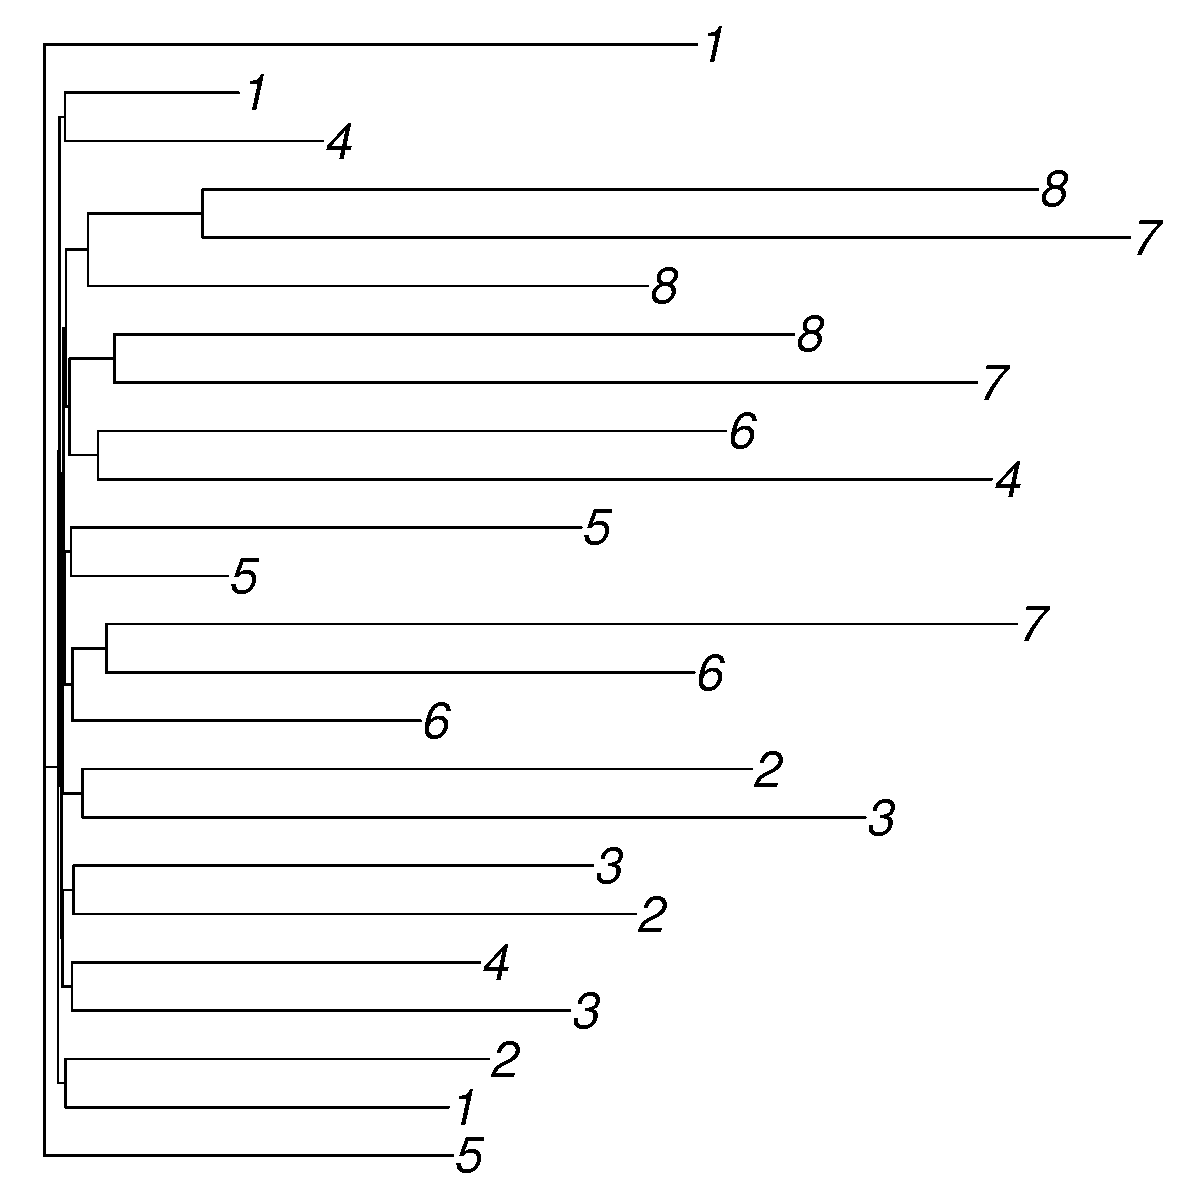
\includegraphics[width=\linewidth]{06-repeat.pdf} &
All 3 replicates match and Only variable sites & 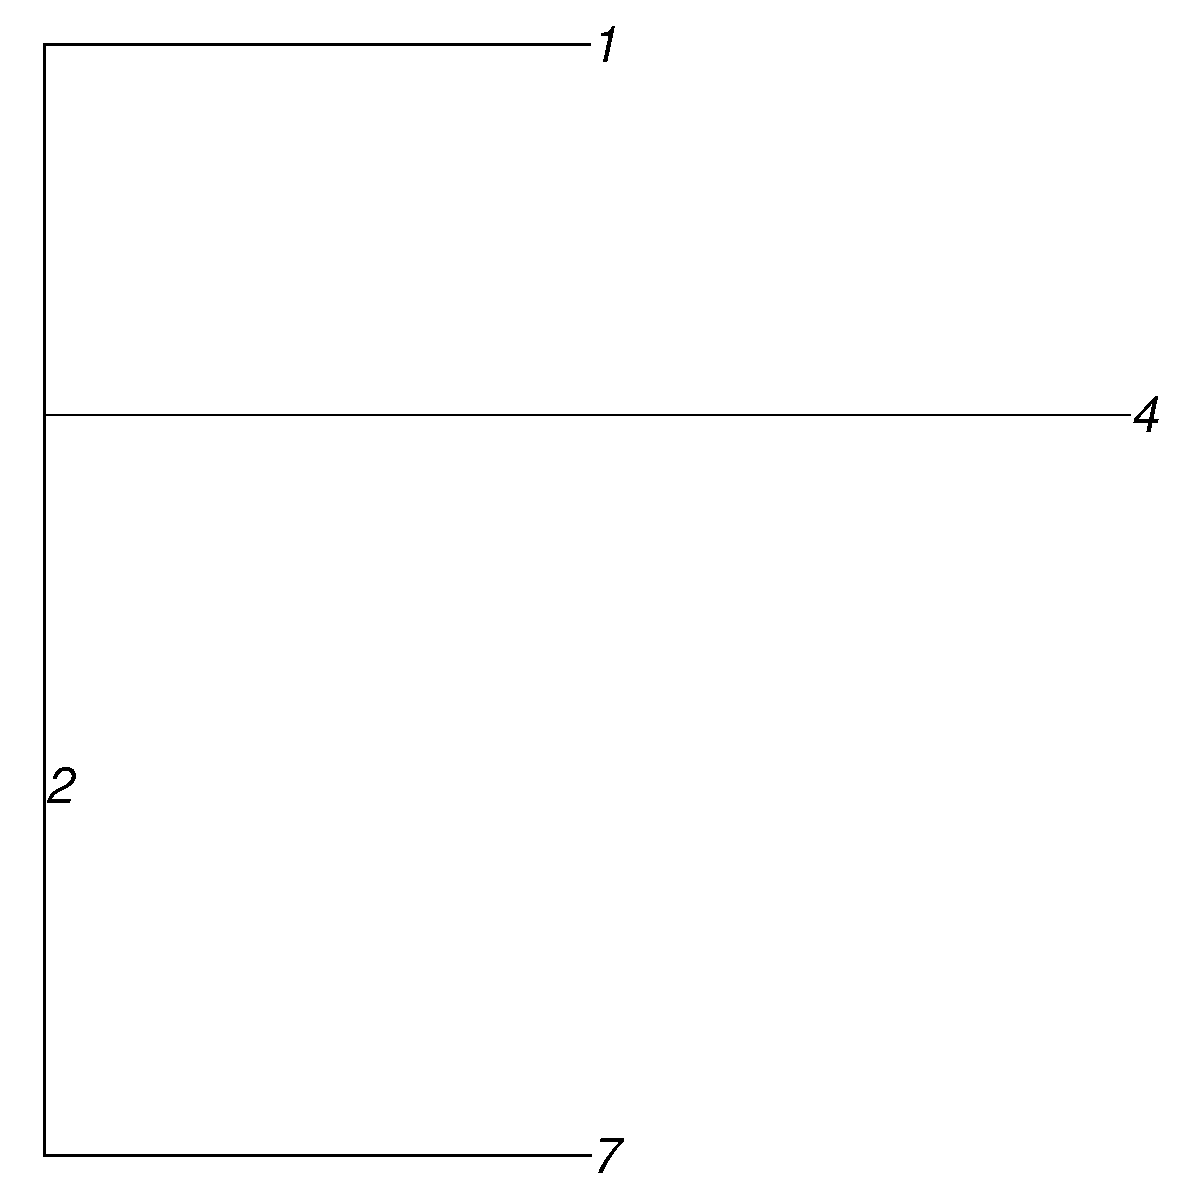
\includegraphics[width=\linewidth]{07-replicate.pdf}\\
% Only variable sites & 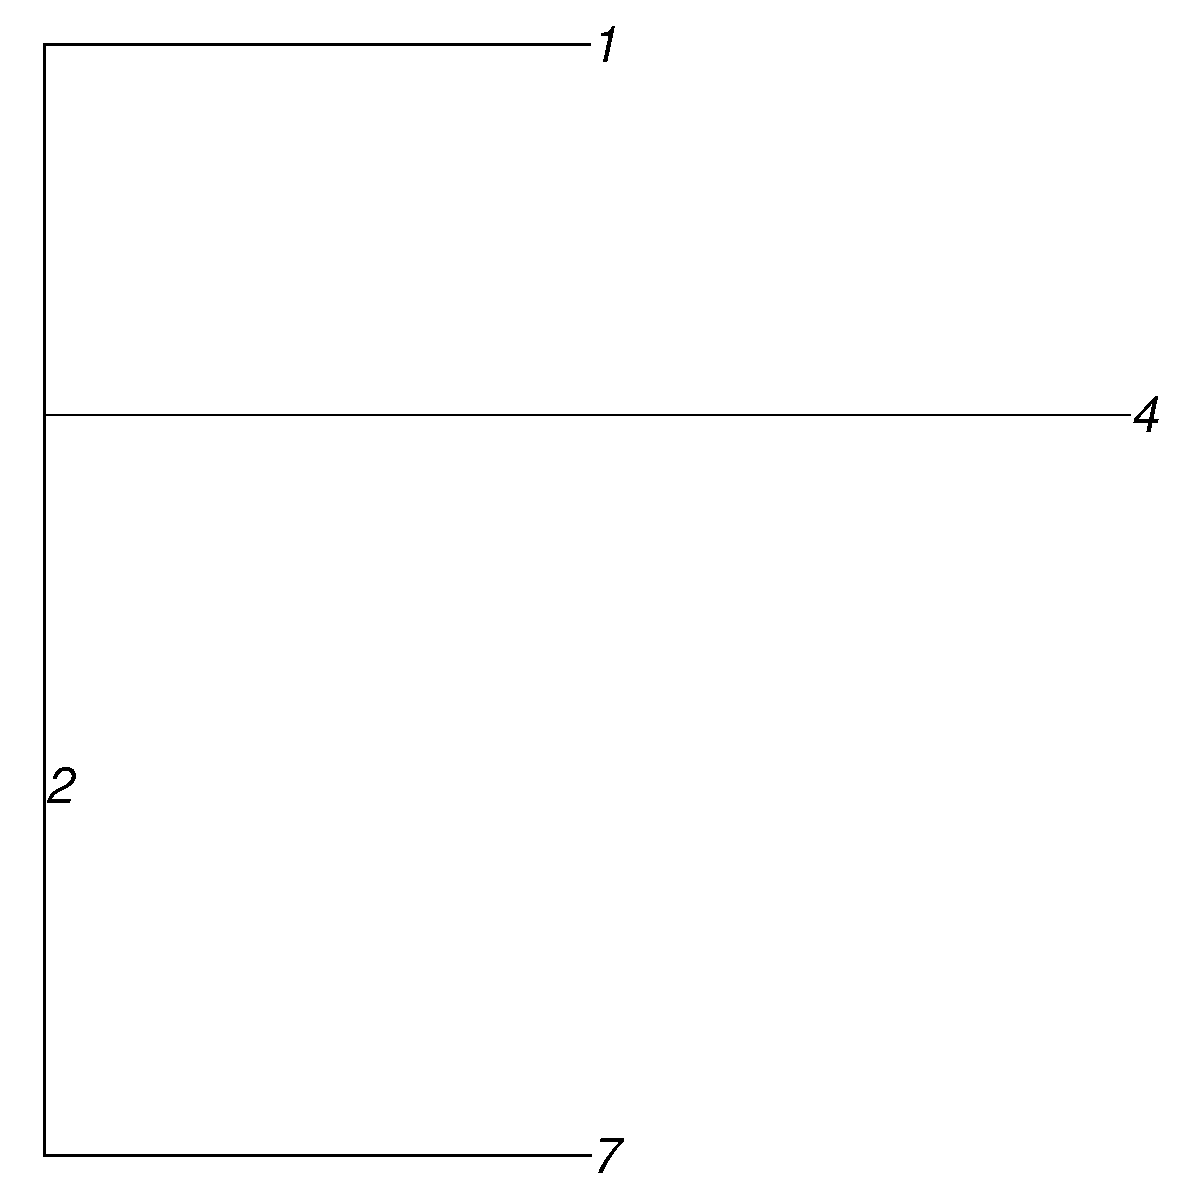
\includegraphics[width=\linewidth]{08-variable.pdf}\\
\bottomrule
\end{tabularx}
\titlecaption{Trees Inferred At Each Filtering Step}{Since each sample was derived from the branch of a tree, its genetic structure should match the physical branching structure. Thus, a phylogeny can visualize the quality of the resultant variant calls; if there are a sufficient number of true positive calls and not many false positives, the phylogeny should match the true structure.}
\label{fig:ev_filtertrees}
\end{figure}

\section{Discussion}

Unfortunately, DiscoSNP++ was not able to accurately detect mutations in this data. There are many fewer detected variants at the start of the filtering pipeline compared to those in \cite{orr_phylogenomic_2020}, with 951,924 variants on the first 11 scaffolds compared to 9,679,544 detected with HaplotypeCaller. This reduced number of potential variants is consistent throughout filtering. However, the number of estimated false positives also remains much lower, with 14.55 after the first filter is applied, in comparison to 1033.18.

At the same time, the estimated trees (Figure \ref{fig:ev_filtertrees}) show a lack of discernable signal that the variant caller is able to capture the tree structure of the data. This seems to contradict the number of false positives found at each step; if there are relatively few false positives, true mutations should drive tree construction and the trees should match the structure of the true tree---or at the very least, replicates of the same sample should be close together on the trees.

However, both tree construction and the procedure for estimating the false positive rate rely on concordance of all replicate genotypes at every site. However, the variant calls emitted by DiscoSNP++ are very sparse, with many sites having at least one missing (./.) genotype. The presence of a missing genotype for any site would eliminate the ability for it to both count as a false positive and contribute useful information during phylogeny construction. Thus, the estimate of the number of false positive sites is artificially deflated, and the number of informative sites in the alignment is small. 

	%todo: make table with number of sites that have at least 1 missing genotype
	%todo: list number of N's in each tree

There are a variety of reasons the algorithm is unable to call genotypes at so many sites. One reason is that the algorithm lacks a reference, so when it detects a variant it may not be able to map it to the genome. For complex or clustered variants, this may be a problem with some samples that doesn't also apply to other samples. This is an especially difficult problem with a repetitive and low-quality genome, such as the one used here. Another major reason is the lack of per-sample depth in this data. Since each replicate was only sequenced to 10X depth, the reads are relatively short, and the genome is repetitive, the de bruijn graph construction may not be well-connected enough to detect variant bubbles. This can very on a per-sample basis as well.

	%todo: try doing the same thing but remove replication to see how increased coverage impacts the number of calls.

\section{Conclusion}

Reference-free variant callers have the potential to be powerful tools for detecting variants in non-model organisms. They are also free of reference bias that may impact other variant callers. However, their performance leaves much to be desired in terms of speed and call accuracy. These callers likely benefit from large per-sample depths and smaller genomes with few repetitive regions. Further development of these methods is warranted.

\printbibliography
